
% ============================================================
%  claude-code-workflow.tex
%  AI-Assisted Research Workflows -- Populism & Narratives
%  Andrea Mentasti & Raffaella Intinghero
%  Wyss Academy for Nature -- April 2026
% ============================================================

\documentclass[aspectratio=169,11pt,dvipsnames]{beamer}

% ---- COLORS ------------------------------------------------
\definecolor{defaultclr}{HTML}{E67E22}
\definecolor{lightgreen}{HTML}{E8F5EE}
\definecolor{darkgreen}{HTML}{0D5032}
\definecolor{codebg}{HTML}{F4F4F4}
\definecolor{alertclr}{HTML}{C0392B}
\definecolor{dropblue}{HTML}{0061FF}

\usecolortheme[named=defaultclr]{structure}

% ---- THEME -------------------------------------------------
\usetheme{Frankfurt}
\setbeamertemplate{navigation symbols}{}
\setbeamertemplate{headline}{}
\setbeamercolor{block title}{fg=white,bg=darkgreen}
\setbeamercolor{block body}{fg=black,bg=lightgreen}
\setbeamercolor{alerted text}{fg=alertclr}

% ---- PACKAGES ----------------------------------------------
\usepackage[T1]{fontenc}
\usepackage[utf8]{inputenc}
\usepackage{lmodern}
\usepackage{amsmath,amssymb}
\usepackage{booktabs}
\usepackage{tcolorbox}
\usepackage{listings}
\usepackage{tikz}
\usetikzlibrary{positioning,arrows.meta,shapes.geometric,fit,backgrounds}
\usepackage{hyperref}
\usepackage{tabularx}
\usepackage{adjustbox}
\usepackage{setspace}
\usepackage{fontawesome5}
\usepackage{url}
\usepackage{fontawesome}

% ---- TCOLORBOX LIBRARY (must include listings) -------------
\tcbuselibrary{skins, listings}

% ---- CODE LISTING STYLE ------------------------------------
% Applied inside codebox via listing options
\lstdefinestyle{codestyle}{
  basicstyle=\scriptsize\ttfamily,
  breaklines=true,
  breakatwhitespace=true,
  numbers=none,
  xleftmargin=0pt,
  xrightmargin=0pt,
  aboveskip=0pt,
  belowskip=0pt,
}

% ---- TCOLORBOX STYLES --------------------------------------
%  codebox: uses newtcblisting so lstlisting is handled
%  natively -- no nesting issues, # characters are safe
\newtcblisting{codebox}[1][]{
  colback=codebg,
  colframe=defaultclr!60,
  fonttitle=\small\bfseries\ttfamily,
  boxrule=0.5pt,
  arc=2pt,
  left=4pt,
  right=4pt,
  top=2pt,
  bottom=2pt,
  listing only,
  listing options={style=codestyle},
  #1
}

\newtcolorbox{greenbox}[1][]{
  colback=lightgreen,
  colframe=darkgreen,
  fonttitle=\bfseries,
  boxrule=0.7pt,
  arc=3pt,
  #1
}

\newtcolorbox{alertbox}[1][]{
  colback=red!8,
  colframe=alertclr,
  colbacktitle=alertclr,
  coltitle=white,
  fonttitle=\bfseries,
  boxrule=0.7pt,
  arc=3pt,
  #1
}

% ---- CUSTOM COMMANDS ---------------------------------------
\newcommand{\skill}[1]{\texttt{\textcolor{defaultclr}{\textbf{/#1}}}}
\newcommand{\file}[1]{\textcolor{darkgreen}{\nolinkurl{#1}}}
\newcommand{\yes}{\textcolor{darkgreen}{\faCheckCircle}}
\newcommand{\no}{\textcolor{alertclr}{\faTimesCircle}}

% ---- TITLE INFO --------------------------------------------
\title{AI-Assisted Research Workflows}
\subtitle{How We Use Claude Code in the Populism \& Narratives Project}
\author{Andrea Mentasti \& Raffaella Intinghero}
\institute{Wyss Academy for Nature}
\date{April 2026}

% ============================================================
\begin{document}
% ============================================================

% ---- SLIDE 1: TITLE ----------------------------------------
\begin{frame}
  \titlepage
  \vspace{-0.5cm}
  \begin{center}
    \small\textit{A practical guide to our project infrastructure}
  \end{center}
\end{frame}

% ============================================================
\section{Why Claude Code?}
% ============================================================

% ---- SLIDE 3: WHAT CLAUDE CODE DOES ------------------------
\begin{frame}{What Claude Code Can Do for Researchers}
\scriptsize
  \begin{columns}[T]
    \begin{column}{0.48\textwidth}
      \textbf{Writing \& running code}
      \begin{itemize}
        \item Python scripts (data prep, classification, figures)
        \item Stata do-files (regressions, tables, plots)
        \item Translates between languages (\skill{script-translator})
      \end{itemize}
      \vspace{0.3cm}
      \textbf{Reviewing code}
      \begin{itemize}
        \item Checks against project conventions
        \item Flags causal language, bad paths, missing labels
        \item \skill{review-stata}, \skill{review-python}
      \end{itemize}
    \end{column}
    \begin{column}{0.48\textwidth}
      \textbf{Managing the project}
      \begin{itemize}
        \item Git branches, commits, pull requests (\skill{commit})
        \item Session logs and quality reports
        \item Literature search (\skill{lit-review})
      \end{itemize}
      \vspace{0.3cm}
      \textbf{Reading documentation}
      \begin{itemize}
        \item Stata PDF manuals (37 volumes, 17\,000 pages)
        \item Extracts relevant sections on demand
        \item No more manual lookups
      \end{itemize}
    \end{column}
  \end{columns}
  \vspace{0.3cm}
  \begin{greenbox}
    \small \textbf{The model:} you direct (``fix the SE clustering''),
    Claude plans and executes. You review the output.
  \end{greenbox}
\end{frame}

% ---- SLIDE 4: THE CONTRACTOR MODEL -------------------------
\begin{frame}{How We Work With Claude}

  \begin{center}
  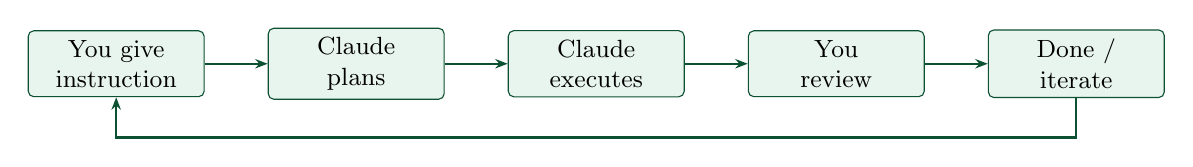
\begin{tikzpicture}[
    node distance=0.2cm and 0.8cm,
    box/.style={rectangle, rounded corners=2pt, draw=darkgreen,
                fill=lightgreen, text width=2cm, align=center,
                minimum height=0.8cm, font=\small},
    arr/.style={-{Stealth[length=4.5pt]}, thick, color=darkgreen}
  ]
    \node[box] (you)  {You give\\ instruction};
    \node[box, right=of you] (plan) {Claude\\ plans};
    \node[box, right=of plan] (exec) {Claude\\ executes};
    \node[box, right=of exec] (rev)  {You\\ review};
    \node[box, right=of rev]  (done) {Done /\\ iterate};

    \draw[arr] (you)  -- (plan);
    \draw[arr] (plan) -- (exec);
    \draw[arr] (exec) -- (rev);
    \draw[arr] (rev)  -- (done);
    \draw[arr] (done.south) -- ++(0,-0.5) -| (you.south);
  \end{tikzpicture}
  \end{center}
  \vspace{0.2cm}
  \begin{columns}[T]
    \begin{column}{0.48\textwidth}
      \textbf{Claude asks you when:}
      \begin{itemize}
        \item Design choices
        \item Presenting a plan
        \item Modifying a .py or .do file
        
      \end{itemize}
    \end{column}
    \begin{column}{0.48\textwidth}
      \textbf{Claude just executes when:}
      \begin{itemize}
        \item Bug fix is obvious
        \item Running a script
        \item Verifying output
        \item Writing session logs
      \end{itemize}
    \end{column}
  \end{columns}
\end{frame}

% ============================================================
\section{Starting Point}
% ============================================================

% ---- SLIDE 5: SANT'ANNA TEMPLATE ---------------------------
\begin{frame}[fragile]{Starting Point: The Sant'Anna Template}
\scriptsize
  \begin{columns}[T]
    \begin{column}{0.58\textwidth}
      We did not build this from scratch.\\[0.4cm]
      \textbf{``My Claude Code Workspace''} is a ready-made
      repository template for research projects. It provides:
      \begin{itemize}
        \item The \file{.claude/} folder structure (rules, skills, agents, hooks)
        \item Workflow templates (session logs, quality reports)
        \item Slide and document utilities
      \end{itemize}
      \vspace{0.3cm}
      \begin{greenbox}[title=Find it at:]
\href{https://psantanna.com/claude-code-my-workflow/workflow-guide.html}{My Claude Code Setup - Pedro H. C. Sant'Anna}
\end{greenbox}
    \end{column}
    \begin{column}{0.38\textwidth}
      \begin{greenbox}[title=What we then customized]
        \begin{itemize}
          \item Rewrote \file{CLAUDE.md} for our project
          \item Added Python \& Stata conventions
          \item Extended hooks to protect raw data
          \item Created the \skill{stata} skill with PDF manual index
          \item Created \skill{script-translator}
        \end{itemize}
      \end{greenbox}
    \end{column}
  \end{columns}
\end{frame}

% ---- SLIDE 6: OUR REPO ------------------------------------
\begin{frame}{Our Project Repository}
  \begin{center}
    \textbf{GitHub repo (template):}
    \url{https://github.com/AndreaMentasti/Claude-Setup---Wyss-Members}
  \end{center}
  \vspace{0.3cm}
  \begin{columns}[T]
    \begin{column}{0.48\textwidth}
      \textbf{Everything in the repo is shared.}\\[0.2cm]
      Any collaborator who clones it gets:
      \begin{itemize}
        \item All rules, skills, agents, hooks
        \item \file{MEMORY.md}, \file{CLAUDE.md}, setup guides
      \end{itemize}
    \end{column}
    \begin{column}{0.48\textwidth}
      \textbf{What is \emph{not} in the repo:}
      \begin{itemize}
        \item Your local config files
        \item API keys
        \item Personal Claude memory
      \end{itemize}
      \vspace{0.2cm}
      \begin{alertbox}[title=Rule 1]
        \small Raw data is \textbf{sacred}. It lives in Dropbox
        and is never committed to git.
      \end{alertbox}
    \end{column}
  \end{columns}
\end{frame}

% ============================================================
\section{The Two-Folder Architecture}
% ============================================================

% ---- SLIDE 7: ARCHITECTURE DIAGRAM -------------------------
\begin{frame}{The Big Picture: Two-Folder Design}
\begin{center}
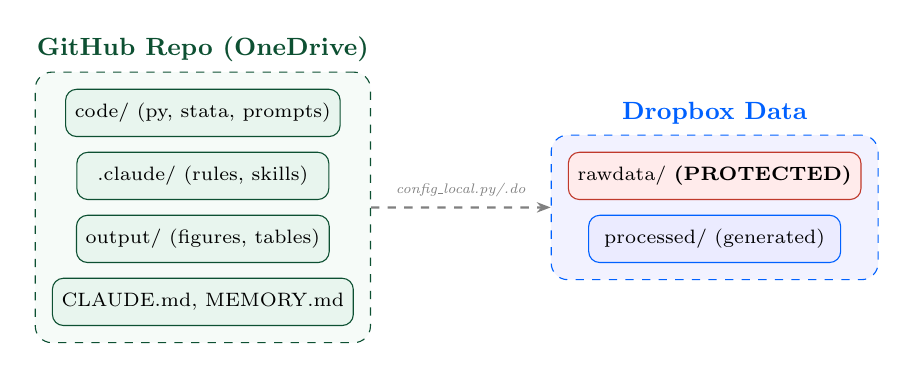
\begin{tikzpicture}[
  every node/.style={font=\scriptsize},
  box/.style={rectangle, rounded corners=4pt, draw, minimum width=3.2cm,
              minimum height=0.6cm, align=center},
  grp/.style={rectangle, rounded corners=6pt, draw, dashed, inner sep=6pt},
  arr/.style={-{Stealth[length=5pt]}, thick}
]
  \node[box, fill=lightgreen, draw=darkgreen] (code)   at (0,2.5) {code/ (py, stata, prompts)};
  \node[box, fill=lightgreen, draw=darkgreen] (claude) at (0,1.7) {.claude/ (rules, skills)};
  \node[box, fill=lightgreen, draw=darkgreen] (output) at (0,0.9) {output/ (figures, tables)};
  \node[box, fill=lightgreen, draw=darkgreen] (docs)   at (0,0.1) {CLAUDE.md, MEMORY.md};

  \begin{scope}[on background layer]
    \node[grp, draw=darkgreen, fill=lightgreen!40,
          fit=(code)(claude)(output)(docs),
          label={[color=darkgreen,font=\bfseries\small]above:GitHub Repo (OneDrive)}] (ghbox) {};
  \end{scope}

  \node[box, fill=red!8, draw=alertclr]  (raw)  at (6.5,1.7) {rawdata/ \textbf{(PROTECTED)}};
  \node[box, fill=blue!8, draw=dropblue] (proc) at (6.5,0.9) {processed/ (generated)};

  \begin{scope}[on background layer]
    \node[grp, draw=dropblue, fill=blue!5,
          fit=(raw)(proc),
          label={[color=dropblue,font=\bfseries\small]above:Dropbox Data}] (dbbox) {};
  \end{scope}

  \draw[arr, color=gray, dashed] (ghbox.east) --
    node[above, font=\tiny\itshape]{config\_local.py/.do} (dbbox.west);
\end{tikzpicture}
\end{center}
\vspace{-0.1cm}
\begin{center}
  \small The repo and Dropbox are \textbf{independent} -- linked only by a
  local config file that is never committed.
\end{center}
\end{frame}

% ---- SLIDE 8: WHAT LIVES WHERE TABLE -----------------------
\begin{frame}{What Lives Where}
  \begin{center}
  \small
  \begin{tabularx}{0.95\textwidth}{lXcc}
    \toprule
    \textbf{Item} & \textbf{Example} & \textbf{GitHub} & \textbf{Dropbox} \\
    \midrule
    Python scripts     & \file{code/py/01_data_prep.py}          & \yes & \no \\
    Stata do-files     & \file{code/stata/1-analysis_main.do}    & \yes & \no \\
    Output figures     & \file{output/figures/fig_engagement.png}& \yes & \no \\
    Rules \& skills    & \file{.claude/rules/project-rules.md}   & \yes & \no \\
    Project memory     & \file{MEMORY.md}, \file{CLAUDE.md}      & \yes & \no \\
    Setup guides       & \file{SETUP.md}, \file{ONBOARDING.md}   & \yes & \no \\
    \midrule
    Raw tweets         & \file{data/rawdata/virality/*.csv}      & \no  & \yes \\
    Processed data     & \file{data/processed/tweets/*.dta}      & \no  & \yes \\
    \midrule
    Local config       & \file{code/py/config_local.py}          & \no  & \no \\      
    Personal memory    & \file{.claude/state/personal-memory.md} & \no  & \no \\
    \bottomrule
  \end{tabularx}
  \end{center}
\end{frame}

\begin{frame}{Why GitHub and Dropbox?}
  \begin{columns}[T]
    \begin{column}{0.48\textwidth}
      \begin{greenbox}[title=\faCheckCircle\ What you gain with GitHub]
        \begin{itemize}\setlength\itemsep{3pt}
        \scriptsize
          \item \textbf{Version history} -- every change recorded with author, date, reason
          \item \textbf{Branches} -- work in parallel without overwriting each other
          \item \textbf{Pull requests} -- review before merging; inline discussion
          \item \textbf{AI integration} -- Claude reads git diff to understand context
          \item \textbf{Rollback} -- restore any past state in seconds
        \end{itemize}
      \end{greenbox}
    \end{column}
    \begin{column}{0.48\textwidth}
      \begin{alertbox}[title=\faExclamationTriangle\ Real trade-offs]
        \begin{itemize}\setlength\itemsep{3pt}
        \scriptsize
          \item \textbf{Learning curve} -- 2--3 hours to get comfortable
          \item \textbf{No binary files} -- large \file{.dta}/\file{.csv} files don't belong in git
          \item \textbf{Conflict resolution} -- if two people edit the same file simultaneously
          \item \textbf{OneDrive + git tension} -- OneDrive locks \file{.git/} files (workaround in \file{SETUP.md})
        \end{itemize}
      \end{alertbox}
    \end{column}
  \end{columns}

\end{frame}

% ============================================================
\section{Git Basics for Economists}
% ============================================================

% ---- SLIDE 10: KEY CONCEPTS ---------------------------------
\begin{frame}{Git Basics}
  \begin{columns}[T]
  \scriptsize
    \begin{column}{0.48\textwidth}
      \begin{tabular}{ll}
        \textbf{Concept} & \textbf{Plain English} \\[4pt]
        \hline\\[-6pt]
        Repository & The project folder, fully tracked \\[3pt]
        Commit      & A saved snapshot with a message \\[3pt]
        Branch      & A parallel version you work on \\[3pt]
        Main        & The official, stable version \\[3pt]
        Pull Request& A proposal to merge into main \\[3pt]
        Clone       & Download the repo to your machine \\[3pt]
        Push/Pull   & Sync local $\leftrightarrow$ GitHub \\[3pt]
      \end{tabular}
    \end{column}
    \begin{column}{0.48\textwidth}
      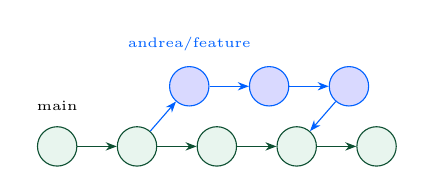
\begin{tikzpicture}[
        node distance=0.5cm,
        c/.style={circle, draw=darkgreen, fill=lightgreen,
                  minimum size=0.5cm, font=\tiny},
        arr/.style={-{Stealth[length=4pt]}, color=darkgreen}
      ]
        \node[c] (m1) {};
        \node[c, right=of m1] (m2) {};
        \node[c, right=of m2] (m3) {};
        \node[c, right=of m3] (m4) {};
        \node[c, right=of m4] (m5) {};
        \draw[arr] (m1)--(m2); \draw[arr] (m2)--(m3);
        \draw[arr] (m3)--(m4); \draw[arr] (m4)--(m5);
        \node[above=2pt of m1, font=\tiny] {main};

        \node[c, fill=blue!15, draw=dropblue,
              above right=0.4cm and 0.3cm of m2] (b1) {};
        \node[c, fill=blue!15, draw=dropblue, right=of b1] (b2) {};
        \node[c, fill=blue!15, draw=dropblue, right=of b2] (b3) {};
        \draw[arr, color=dropblue] (m2)--(b1);
        \draw[arr, color=dropblue] (b1)--(b2);
        \draw[arr, color=dropblue] (b2)--(b3);
        \draw[arr, color=dropblue] (b3)--(m4);
        \node[above=2pt of b1, font=\tiny, color=dropblue] {andrea/feature};
      \end{tikzpicture} \\
      \vspace{0.2cm}
      \scriptsize A branch lets you develop a feature without touching
      \texttt{main}. When ready, open a PR and merge it back.
    \end{column}
  \end{columns}
\end{frame}

% ---- SLIDE 11: DAILY WORKFLOW ------------------------------
\begin{frame}[fragile]{The Daily Git Workflow}
\scriptsize
  \begin{enumerate}\setlength\itemsep{6pt}
    \item \textbf{Pull latest main} before starting:
      \begin{codebox}
git checkout main
git pull origin main
      \end{codebox}
    \item \textbf{Create your branch}:
      \begin{codebox}
git checkout -b andrea/openai-stage3-fix
      \end{codebox}
    \item \textbf{Work.} Commit small logical chunks:
      \begin{codebox}
git add code/py/my_script.py
git commit -m "fix stage3 prompt template"
      \end{codebox}
    \item \textbf{Push and open a Pull Request} on GitHub.
    \item \textbf{After merge:} pull main, delete your branch.
  \end{enumerate}
  \vspace{0.2cm}
  \begin{greenbox}
    \scriptsize \textbf{Shortcut:} use \skill{commit} OR ask Claude Code in natural language -- Claude stages, writes the message,
    creates the PR, and merges, all in one command.
  \end{greenbox}
\end{frame}

% ---- SLIDE 12: BRANCH NAMING + CONFLICT AVOIDANCE ----------
\begin{frame}[fragile]{Branch Naming \& Avoiding Conflicts}
  \begin{columns}[T]
    \begin{column}{0.46\textwidth}
    \scriptsize
      \textbf{Branch naming convention}\\[4pt]
      Always prefix with your name:
      \begin{codebox}
andrea/openai-stage3-fix
andrea/visibrain-cleanup
raffaella/stata-event-study
raffaella/politician-analysis
      \end{codebox}
      Why: instant clarity on who owns what.
    \end{column}
    \begin{column}{0.50\textwidth}
    \scriptsize
      \textbf{Conflict avoidance rules}
      \begin{itemize}\setlength\itemsep{4pt}
        \item \textbf{Always pull main before branching} -- stale starts are the main cause of conflicts
        \item \textbf{Never push directly to main} -- always branch + Pull Request
        \item \textbf{Coordinate} before editing \file{CLAUDE.md} or \file{project-rules.md}
        \item \textbf{One merge at a time} -- if both have open PRs, merge one, pull, then merge the other
      \end{itemize}
    \end{column}
  \end{columns}
  \vspace{0.3cm}
    \begin{greenbox}
    \scriptsize \textbf{If you get a merge conflict:} Git marks conflicting sections.
    Edit the file to keep the right version, then \texttt{git add} and \texttt{git commit}.
    See \file{COLLABORATION.md} for step-by-step instructions.
  \end{greenbox}
\end{frame}

% ============================================================
\section{One-Time Setup: Project Owner}
% ============================================================

% ---- SLIDE 14: OWNER SETUP OVERVIEW -------------------------
\begin{frame}{Step 0 — Before Your Colleagues Join: Owner Setup}
\scriptsize
  Two kinds of setup exist: \textbf{owner} (once, to adapt the template) and
  \textbf{collaborator} (once per machine, to join the project).
  \vspace{0.2cm}
  \begin{columns}[T]
    \begin{column}{0.52\textwidth}
      \textbf{Owner: 4 steps, $\sim$30 minutes}
      \begin{enumerate}\setlength\itemsep{5pt}
        \item \textbf{Clone the template}
          \begin{codebox}
git clone https://github.com/AndreaMentasti/
  Claude-Setup---Wyss-Members.git your_project
          \end{codebox}
        \item \textbf{Fill 4 placeholders} (find \& replace across repo):
          \begin{codebox}
[YOUR_PROJECT_NAME]   -> e.g. My Research Project
[YOUR_INSTITUTION]    -> e.g. Wyss Academy
[YOUR_GITHUB_REPO_URL]-> your repo URL
[YOUR_REPO_NAME]      -> your repo name
          \end{codebox}
        \item \textbf{Customize 3 key files} (next slide)
        \item \textbf{Push to your project repo + invite collaborators}
          \begin{codebox}
git remote set-url origin https://github.com/you/repo
git push -u origin main
          \end{codebox}
      \end{enumerate}
    \end{column}
    \begin{column}{0.44\textwidth}
      \begin{greenbox}[title=Files with placeholders to fill]
        \small
        \begin{itemize}
          \item \file{CLAUDE.md}
          \item \file{ONBOARDING.md}
          \item \file{COLLABORATION.md}
          \item \file{MEMORY.md}
        \end{itemize}
      \end{greenbox}
      \vspace{0.3cm}
      \begin{alertbox}[title=Do this before sharing the repo]
        \small Collaborators who clone \textbf{before} you fill the
        placeholders will see \texttt{[YOUR\_PROJECT\_NAME]}
        everywhere. Fill first, then invite.
      \end{alertbox}
    \end{column}
  \end{columns}
\end{frame}

% ---- SLIDE 15: THREE FILES TO CUSTOMIZE ----------------------
\begin{frame}{Step 0 — The Three Files to Customize}
\scriptsize
  Everything else works out of the box. Only these three need your attention:
  \vspace{0.2cm}
  \begin{columns}[T]
    \begin{column}{0.33\textwidth}
      \begin{greenbox}[title=1. CLAUDE.md]
        Update two sections:
        \begin{itemize}
          \item \textbf{Folder structure} tree --- reflect your actual data layout
          \item \textbf{Pipeline state} table --- list your actual scripts and stages
        \end{itemize}
        \vspace{0.2cm}
        Claude reads this every session.
        Everything else is already correct.
      \end{greenbox}
    \end{column}
    \begin{column}{0.33\textwidth}
      \begin{greenbox}[title=2. project-rules.md]
        Update \textbf{Rule 1} only:\\
        replace the example rawdata subfolder names with
        your actual folder names.\\[0.3cm]
        Rules 2--7 are generic and need no changes.
      \end{greenbox}
    \end{column}
    \begin{column}{0.30\textwidth}
      \begin{alertbox}[title=\faExclamationTriangle\ 3. domain-reviewer.md]
        \small \textbf{Most important.} Rewrite the 5 review lenses
        for your research field:
        \begin{itemize}
          \item Research design
          \item Data validity
          \item Citation fidelity
          \item Code--theory alignment
          \item Causal claims
        \end{itemize}
        This makes review domain-aware.
        Takes $\sim$20 min.
      \end{alertbox}
    \end{column}
  \end{columns}
  \vspace{0.2cm}
  \begin{center}
    \small \textbf{Optional:} delete slide-related skills if your project
    does not use LaTeX/Quarto (see \file{ONBOARDING.md} for the list).
  \end{center}
\end{frame}

% ============================================================
\section{One-Time Setup: Collaborators}
% ============================================================

% ---- SLIDE 16: PREREQUISITES --------------------------------
\begin{frame}{What Each Collaborator Needs}
  \begin{columns}[T]
  \scriptsize
    \begin{column}{0.48\textwidth}
      \textbf{Accounts and access:}
      \begin{itemize}
        \item GitHub account — collaborator invite from the project owner
        \item Shared data folder (Dropbox / SharePoint / OneDrive)\\
              synced to your machine
        \item Anthropic account — for Claude Code
      \end{itemize}
      \vspace{0.3cm}
      \textbf{Software to install:}
      \begin{itemize}
        \item Git
        \item Python 3.10+
        \item Stata (if using Stata scripts)
        \item Claude Code desktop app
        \item GitHub Desktop (optional, but easier)
      \end{itemize}
    \end{column}
    \begin{column}{0.48\textwidth}
      \begin{greenbox}[title=\faLightbulb\ The onboarding shortcut]
        Once Claude Code is open and the repo is cloned,
        \textbf{you do not set anything up manually}.\\[0.4cm]
        Paste one prompt into Claude Code and it
        configures your entire environment automatically:\\[0.2cm]
        \begin{itemize}
          \item Config files
          \item Python dependencies
          \item Stata on PATH
          \item Git identity
          \item Compound Engineering plugin
        \end{itemize}
        See next slide.
      \end{greenbox}
    \end{column}
  \end{columns}
\end{frame}

% ---- SLIDE 17: THE MAGIC PROMPT ----------------------------
\begin{frame}[fragile]{The Onboarding Prompt: Claude Does the Rest}
  \begin{codebox}[title=Paste into Claude Code -- fill in the three bracketed fields]
I am a new collaborator on [PROJECT NAME].
- OS: [Windows / Mac]
- My shared data folder: [e.g. C:\Users\YourName\Dropbox\your_project\data]
- Stata version and location: [e.g. Stata 17 at C:\Program Files\Stata17]

Please set up my environment completely:
1. Read CLAUDE.md to understand the project structure.
2. Create config_local.py and config_local.do from the templates.
   Set DATA_ROOT / data_root to my data folder above.
3. Install Python dependencies (pip install -r requirements.txt + pdfplumber).
4. Add Stata to my system PATH.
5. Set my git identity (ask me for name and email).
6. Install the Compound Engineering plugin.
7. Create .claude/state/personal-memory.md with my machine details.
8. Verify: run python -c "import config; print(config.DATA_RAW)"
   and stata -e version. Report any errors.
  \end{codebox}
  \vspace{0.1cm}
  \small \textbf{Claude will ask your name and email, then handle everything else.}
  The full prompt text is in \file{ONBOARDING.md}.
\end{frame}

% ---- SLIDE 18: CONFIG FILES --------------------------------
\begin{frame}[fragile]{The Config Bridge: Connecting Code to Data}
  \begin{center}
  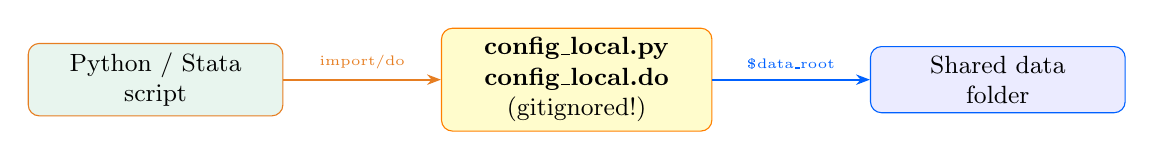
\begin{tikzpicture}[
    node distance=0.5cm and 1.5cm,
    box/.style={rectangle, rounded corners, draw, minimum height=0.7cm,
                align=center, font=\small},
    arr/.style={-{Stealth[length=5pt]}, thick}
  ]
    \node[box, fill=lightgreen, draw=defaultclr, text width=3cm] (script)
      {Python / Stata\\ script};
    \node[box, fill=yellow!20, draw=orange, text width=3.2cm, right=2cm of script] (cfg)
      {\textbf{config\_local.py}\\ \textbf{config\_local.do}\\ \small (gitignored!)};
    \node[box, fill=blue!8, draw=dropblue, text width=3cm, right=2cm of cfg] (data)
      {Shared data\\ folder};

    \draw[arr, color=defaultclr] (script) -- node[above,font=\tiny]{import/do} (cfg);
    \draw[arr, color=dropblue]   (cfg)    -- node[above,font=\tiny]{\$data\_root} (data);
  \end{tikzpicture}
  \end{center}
  \vspace{0.3cm}
  \begin{columns}[T]
    \begin{column}{0.48\textwidth}
      \textbf{Python} -- \file{code/py/config_local.py}
      \begin{codebox}
DATA_ROOT = Path(
  r"C:\Users\YourName\Dropbox\your_project\data"
)
      \end{codebox}
    \end{column}
    \begin{column}{0.48\textwidth}
      \textbf{Stata} -- \file{code/stata/config_local.do}
      \begin{codebox}
global data_root ///
  "C:/Users/YourName/Dropbox/your_project/data"
global root "C:/path/to/your_project"
      \end{codebox}
    \end{column}
  \end{columns}
  \vspace{0.2cm}
  \begin{alertbox}
    \small These files are \textbf{gitignored} -- they never appear in
    \texttt{git status} and are never committed.
    Each collaborator creates their own from a template.
  \end{alertbox}
\end{frame}

% ---- SLIDE 19: VERIFY --------------------------------------
\begin{frame}[fragile]{Verify Your Setup}
  \begin{columns}[T]
    \begin{column}{0.55\textwidth}
      \textbf{Run these checks after setup:}
      \begin{codebox}
\# 1. Config points to your data folder:
python -c "import sys; sys.path.insert(0,'code/py'); \
  import config; print(config.DATA_RAW)"

\# 2. Stata is on PATH:
stata -e version

\# 3. No config_local files in git:
git status

\# 4. Plugin installed:
claude skills list
      \end{codebox}
    \end{column}
    \begin{column}{0.41\textwidth}
      \textbf{If something breaks:}\\[0.3cm]
      Paste the error into Claude Code:
      \begin{codebox}
I got this error during setup:
[paste full error message]
Please diagnose and fix it.
      \end{codebox}
      \vspace{0.2cm}
      \begin{greenbox}
        \small Claude traces the cause and fixes it.
        This is faster than reading a stack trace yourself.
      \end{greenbox}
    \end{column}
  \end{columns}
\end{frame}

% ---- SLIDE 20: WHAT GETS INSTALLED -------------------------
\begin{frame}{What the Onboarding Prompt Actually Installs}
\scriptsize
  \begin{columns}[T]
    \begin{column}{0.48\textwidth}
      \begin{greenbox}[title=Compound Engineering Plugin]
        \small
        A Claude Code plugin by EveryInc that adds advanced skills.\\[0.3cm]
        \textbf{Install with:}\\
        \texttt{claude plugin marketplace add}\\
        \texttt{EveryInc/compound-engineering-plugin}\\[0.3cm]
        \textbf{What it enables:}
        \begin{itemize}
          \item \skill{commit} -- the main daily driver
          \item \skill{ce-plan}, \skill{ce-work}, \skill{ce-review}
          \item \skill{deep-audit}, \skill{learn}
        \end{itemize}
        \textbf{Required?} Yes -- without it \skill{commit} does not work.\\
        \textbf{Cost?} Free. The onboarding prompt runs it automatically.
      \end{greenbox}
    \end{column}
    \begin{column}{0.48\textwidth}
      \begin{greenbox}[title=PDF Reading Tools (Stata manuals)]
        \small
        Claude can consult Stata's bundled PDF manuals
        (37 volumes, 17\,000 pages) when writing \file{.do} files.\\[0.3cm]
        \textbf{pdfplumber} (Python library)\\
        \quad Reads tables from PDFs.\\
        \quad Auto-installed via \texttt{requirements.txt} -- nothing to do.\\[0.3cm]
        \textbf{pdftotext} (command-line tool)\\
        \quad \textbf{Windows:} already bundled with Git for Windows.\\
        \quad \textbf{Mac:} \texttt{brew install poppler} (one command).\\[0.3cm]
        \textbf{Required?} Only if using Stata with the \skill{stata} skill.
        Can be skipped otherwise.
      \end{greenbox}
    \end{column}
  \end{columns}
\end{frame}

% ============================================================
\section{The Intelligence Layer}
% ============================================================

% ---- SLIDE 21: CLAUDE.MD -----------------------------------
\begin{frame}{\file{CLAUDE.md}: The Project Brain}
  \begin{columns}[T]
    \begin{column}{0.55\textwidth}
      \file{CLAUDE.md} is loaded by Claude Code \textbf{at the start of every session}.
      It tells Claude:
      \begin{itemize}\setlength\itemsep{4pt}
        \item What this project is (research question, team, institution)
        \item The folder structure (repo vs.\ shared data)
        \item Which config module to use (\texttt{import config as cfg})
        \item All available slash commands
        \item The current pipeline state (what is done, what is next)
        \item Quality thresholds (80 to commit, 90 for PR)
      \end{itemize}
      \vspace{0.2cm}
      Think of it as the \textbf{standing brief} that every new session reads first.
    \end{column}
    \begin{column}{0.41\textwidth}
      \begin{greenbox}[title=Practical implication]
        \small If you pull a change that modifies \file{CLAUDE.md}
        or \file{.claude/} mid-session, \textbf{start a new Claude
        Code session} to pick up the changes.
      \end{greenbox}
      \vspace{0.3cm}
      \begin{block}{Amendment protocol}
        \small To change a rule or convention:
        \begin{enumerate}
          \item Say ``I want to amend Rule N''
          \item Claude asks: permanent or one-time?
          \item Edit the file explicitly
        \end{enumerate}
      \end{block}
    \end{column}
  \end{columns}
\end{frame}

% ---- SLIDE 22: RULES ---------------------------------------
\begin{frame}{Rules: Non-Negotiable Guardrails}
  Located in \file{.claude/rules/} -- loaded every session. Seven hard rules:

  \begin{columns}[T]
    \begin{column}{0.48\textwidth}
      \begin{enumerate}\setlength\itemsep{4pt}
        \item \textbf{Raw data is sacred} -- never overwrite \file{data/rawdata/}
        \item \textbf{Correlational framing} -- no causal language without an identification strategy
        \item \textbf{All paths via config} -- no hardcoded absolute paths anywhere
        \item \textbf{Publication-ready figures} -- PNG, 300 DPI, white background
      \end{enumerate}
    \end{column}
    \begin{column}{0.48\textwidth}
      \begin{enumerate}\setlength\itemsep{4pt}
        \setcounter{enumi}{4}
        \item \textbf{Scripts must run clean} -- exit code 0 before committing
        \item \textbf{\file{old/} folders are read-only} -- never modify archives
        \item \textbf{Ask before modifying scripts} -- Claude states what it will change and waits for confirmation
      \end{enumerate}
    \end{column}
  \end{columns}
  \vspace{0.3cm}
  \begin{greenbox}
    \small \textbf{Beyond the 7 rules:} \file{.claude/rules/} also contains
    Python conventions, Stata conventions, session-logging protocol,
    and the plan-first workflow. These govern \emph{how} Claude works,
    not just what it protects.
  \end{greenbox}
\end{frame}

% ---- SLIDE 23: SKILLS --------------------------------------
\begin{frame}{Skills: Custom Slash Commands}
  Skills are Claude's \textbf{pre-programmed workflows}. Type a \texttt{/} command
  and Claude executes a multi-step protocol automatically.

  \vspace{0.3cm}
  \begin{columns}[T]
    \begin{column}{0.48\textwidth}
      \textbf{Analysis \& code}
      \begin{itemize}
        \item \skill{data-analysis} -- end-to-end workflow
        \item \skill{review-python} \skill{review-stata} -- quality review
        \item \skill{script-translator} -- port code between Python / Stata / R
        \item \skill{stata} -- loads Stata PDF manual index
      \end{itemize}
      \vspace{0.2cm}
      \textbf{Git \& project management}
      \begin{itemize}
        \item \skill{commit} -- stage, message, PR, merge
        \item \skill{context-status} -- check session health
      \end{itemize}
    \end{column}
    \begin{column}{0.48\textwidth}
      \textbf{Research}
      \begin{itemize}
        \item \skill{lit-review} -- structured literature search
        \item \skill{research-ideation} -- generate hypotheses
        \item \skill{interview-me} -- interactive specification
        \item \skill{review-paper} -- manuscript critique
      \end{itemize}
      \vspace{0.2cm}
      \textbf{From the Compound Engineering plugin}
      \begin{itemize}
        \item \skill{ce-plan}, \skill{ce-work}, \skill{ce-review}
        \item \skill{deep-audit}, \skill{deepen-plan}
      \end{itemize}
    \end{column}
  \end{columns}
  \vspace{0.2cm}
  \small Skills live in \file{.claude/skills/} -- every collaborator gets them automatically on clone.
\end{frame}

% ---- SLIDE 24: AGENTS --------------------------------------
\begin{frame}{Agents: Specialized Reviewers}
  Agents are autonomous sub-processes Claude launches for focused analysis.
  They live in \file{.claude/agents/} and run when Claude decides they are needed.

  \vspace{0.3cm}
  \begin{columns}[T]
    \begin{column}{0.48\textwidth}
      \textbf{Domain-specific agents}
      \begin{itemize}
        \item \texttt{domain-reviewer} -- flags causal language, checks research design, validates citations \textbf{(customize this)}
        \item \texttt{stata-reviewer} -- reviews \file{.do} files for conventions, pitfalls, reproducibility
        \item \texttt{python-reviewer} -- pandas idioms, path conventions, output standards
        \item \texttt{r-reviewer} -- for R scripts
      \end{itemize}
    \end{column}
    \begin{column}{0.48\textwidth}
      \textbf{Quality agents}
      \begin{itemize}
        \item \texttt{proofreader} -- grammar, typos, consistency
        \item \texttt{verifier} -- checks scripts compile and run
        \item \texttt{slide-auditor} -- overflow, font consistency
        \item \texttt{beamer-translator} -- Beamer to Quarto
      \end{itemize}
      \vspace{0.3cm}
      \begin{greenbox}
        \small Agents give \textbf{reports with proposed changes} and wait for
        your approval before editing any file. You stay in control.
      \end{greenbox}
    \end{column}
  \end{columns}
\end{frame}

% ---- SLIDE 25: MEMORY & HOOKS ------------------------------
\begin{frame}{Memory and Hooks}
  \begin{columns}[T]
    \begin{column}{0.48\textwidth}
      \textbf{Two-tier memory system}\\[4pt]
      \begin{tabular}{p{2cm}p{3.5cm}}
        \small\file{MEMORY.md} & \small Project knowledge, committed, shared across all collaborators \\[6pt]
        \small\file{.claude/state/personal-memory.md} & \small Your machine-specific setup (gitignored, local only) \\
      \end{tabular}
      \vspace{0.3cm}
      \file{MEMORY.md} is loaded every session. It contains:
      \begin{itemize}
        \item Pipeline decisions and rationale
        \item Workflow lessons learned
        \item Progress log (session by session)
      \end{itemize}
      \small Add entries with \texttt{[LEARN:category]} when Claude is corrected.
    \end{column}
    \begin{column}{0.48\textwidth}
      \textbf{Hooks: automated checks}\\[4pt]
      Scripts that fire automatically at key moments:
      \begin{itemize}\setlength\itemsep{4pt}
        \item \textbf{verify-reminder} -- after editing any \file{.py} or \file{.do} file, reminds Claude to run and verify it
        \item \textbf{protect-files} -- blocks writes to \file{rawdata/} at the tool level; enforces Rule 1
        \item \textbf{pre-compact} -- before context compression, saves session state to disk
        \item \textbf{post-compact-restore} -- after compression, re-reads plan and states next step
        \item \textbf{context-monitor} -- warns when context usage is high
        \item \textbf{log-reminder} -- prompts Claude to update the session log
      \end{itemize}
    \end{column}
  \end{columns}
\end{frame}

% ============================================================
\section{Daily Workflow}
% ============================================================

% ---- SLIDE 26: SESSION START --------------------------------
\begin{frame}[fragile]{Starting a Work Session}
  \begin{columns}[T]
    \begin{column}{0.55\textwidth}
      \textbf{Step 1: Pull latest main}
      \begin{codebox}
git checkout main
git pull origin main
      \end{codebox}
      \textbf{Step 2: Create your branch}
      \begin{codebox}
git checkout -b yourname/task-description
      \end{codebox}
      \textbf{Step 3: Open Claude Code, open the folder}\\
      Claude reads \file{CLAUDE.md} and all rules automatically.\\[0.3cm]
      \textbf{Step 4: Tell Claude your task}
      \begin{codebox}
Run code/stata/your_analysis.do
and show me any errors from the log.
      \end{codebox}
    \end{column}
    \begin{column}{0.41\textwidth}
      \begin{greenbox}[title=Useful daily prompts]
        \small
        \textbf{Review before committing:}\\
        \texttt{/review-stata code/stata/analysis.do}\\[0.3cm]
        \textbf{Fix an error:}\\
        \textit{I got this error: [paste]. Fix it.}\\[0.3cm]
        \textbf{Commit and PR:}\\
        \texttt{/commit}\\[0.3cm]
        \textbf{See what changed:}\\
        \textit{Show me what I changed since last commit.}\\[0.3cm]
        \textbf{Translate a script:}\\
        \texttt{/script-translator}
      \end{greenbox}
    \end{column}
  \end{columns}
\end{frame}

% ---- SLIDE 27: WORKING WITH STATA --------------------------
\begin{frame}[fragile]{Working With Stata: The \skill{stata} Skill}
  \begin{columns}[T]
    \begin{column}{0.55\textwidth}
      \textbf{What \skill{stata} gives Claude}
      \begin{itemize}\setlength\itemsep{4pt}
        \item A full index of Stata's \textbf{37 PDF manuals}
          (17\,000 pages, installed with Stata)
        \item A strategy for reading them efficiently:
          \texttt{pdftotext} for prose sections,
          \texttt{pdfplumber} for tables
        \item Stata-specific patterns: \texttt{estout}/\texttt{esttab},
          \texttt{binsreg}, event studies, \texttt{ivreg2}
        \item Common pitfalls (missing values, factor variables,
          \texttt{=} vs.\ \texttt{==}, local macro syntax)
      \end{itemize}
      \vspace{0.2cm}
      \textbf{Running Stata from Claude:}
      \begin{codebox}
Run code/stata/your_analysis.do
and check the log for errors.
      \end{codebox}
    \end{column}
    \begin{column}{0.41\textwidth}
      \begin{greenbox}[title=Example interactions]
        \small
        \textit{``How do I produce a grouped bar chart in Stata
        with a color legend?''}\\[0.2cm]
        Claude reads the relevant PDF sections and returns
        working code -- citing the exact page.\\[0.3cm]
        \textit{``Translate this Python regression to Stata.''}\\[0.2cm]
        \skill{script-translator} handles it line by line,
        with Stata idioms.
      \end{greenbox}
      \vspace{0.2cm}
      \small \textbf{Quality gate:} \skill{review-stata} checks all
      Stata conventions in your \file{.do} file before you commit.
    \end{column}
  \end{columns}
\end{frame}

% ---- SLIDE 28: COMMITTING WITH /COMMIT ---------------------
\begin{frame}{Committing: The \skill{commit} Skill}
  Instead of running git commands manually, just type:
  \begin{center}
    \Large\texttt{/commit}
  \end{center}
  Claude then:
  \begin{enumerate}\setlength\itemsep{4pt}
    \item Runs \texttt{git status} and \texttt{git diff} to see what changed
    \item Drafts a commit message focused on \emph{why} (not just what)
    \item Stages the relevant files (\textbf{never} \texttt{git add .})
    \item Creates the commit, pushes the branch
    \item Opens a Pull Request on GitHub with a structured summary
    \item (Optionally) merges the PR if you approve
  \end{enumerate}
  \vspace{0.2cm}
  \begin{alertbox}
    \small Claude will \textbf{never push to main directly} and will \textbf{never commit
    \file{config_local.*} or \file{.env} files}. These guardrails are baked into the skill.
  \end{alertbox}
\end{frame}

% ============================================================
\section{Personalizing the Setup}
% ============================================================

% ---- SLIDE 29: HOW TO CUSTOMIZE ---------------------------
\begin{frame}[fragile]{Personalizing: Make It Your Own}
  \begin{columns}[T]
    \begin{column}{0.48\textwidth}
      \textbf{What you can customize}
      \begin{itemize}\setlength\itemsep{4pt}
        \item \file{CLAUDE.md} -- update pipeline state, add your role, adjust quality thresholds
        \item \file{.claude/rules/} -- add new rules, amend existing ones
        \item \file{.claude/skills/} -- write new slash commands for recurring tasks
        \item \file{MEMORY.md} -- add project knowledge after each session
        \item \file{.claude/state/personal-memory.md} -- your machine-specific notes
      \end{itemize}
    \end{column}
    \begin{column}{0.48\textwidth}
      \textbf{Add a new rule}\\[4pt]
      Create \file{.claude/rules/my-rule.md}:
      \begin{codebox}
\# My Custom Rule

Never use `merge` without checking
`_merge` distribution first.
Always run: tab _merge
      \end{codebox}
      Loaded automatically next session.\\[0.3cm]
      \textbf{Add a new skill}\\[4pt]
      Create \file{.claude/skills/my-skill/SKILL.md}\\
      and type \texttt{/my-skill} in Claude Code.
    \end{column}
  \end{columns}
\end{frame}

% ---- SLIDE 30: ARCHITECTURE + GET STARTED ------------------
\begin{frame}{The Architecture at a Glance}
\begin{center}
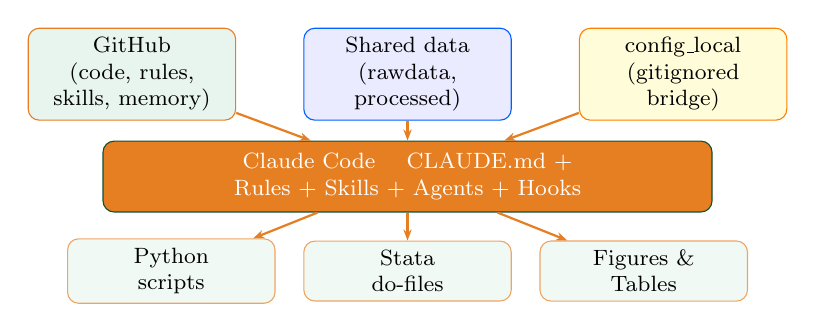
\begin{tikzpicture}[
  every node/.style={font=\footnotesize},
  box/.style={rectangle, rounded corners=4pt, draw, align=center,
              minimum height=0.65cm},
  arr/.style={-{Stealth[length=4pt]}, thick, color=defaultclr}
]
  \node[box, fill=lightgreen, draw=defaultclr, text width=2.4cm] (gh)
    at (0, 2.5) {GitHub\\ (code, rules,\\ skills, memory)};
  \node[box, fill=blue!8, draw=dropblue, text width=2.4cm] (db)
    at (3.5, 2.5) {Shared data\\ (rawdata,\\ processed)};
  \node[box, fill=yellow!15, draw=orange, text width=2.4cm] (cfg)
    at (7, 2.5) {config\_local\\ (gitignored bridge)};

  \node[box, fill=defaultclr, text=white, draw=darkgreen, text width=7.5cm,
        minimum height=0.9cm] (cc)
    at (3.5, 1.2) {Claude Code
      \quad CLAUDE.md + Rules + Skills + Agents + Hooks};

  \node[box, fill=lightgreen!60, draw=defaultclr!70, text width=2.4cm] (py)
    at (0.5, 0) {Python\\ scripts};
  \node[box, fill=lightgreen!60, draw=defaultclr!70, text width=2.4cm] (st)
    at (3.5, 0) {Stata\\ do-files};
  \node[box, fill=lightgreen!60, draw=defaultclr!70, text width=2.4cm] (out)
    at (6.5, 0) {Figures \&\\ Tables};

  \draw[arr] (gh)  -- (cc);
  \draw[arr] (db)  -- (cc);
  \draw[arr] (cfg) -- (cc);
  \draw[arr] (cc)  -- (py);
  \draw[arr] (cc)  -- (st);
  \draw[arr] (cc)  -- (out);
\end{tikzpicture}
\end{center}
\vspace{0.1cm}
\begin{columns}[T]
  \begin{column}{0.48\textwidth}
    \begin{greenbox}[title=Template repo]
      \small \url{https://github.com/AndreaMentasti/Claude-Setup---Wyss-Members}
    \end{greenbox}
  \end{column}
  \begin{column}{0.48\textwidth}
    \begin{center}
      \small \textbf{Clone. Fill placeholders. Customize 3 files.}\\
      \textbf{Push. Invite collaborators.}\\[0.2cm]
      \textbf{Welcome to the project.}
    \end{center}
  \end{column}
\end{columns}
\end{frame}

% ============================================================
\end{document}
